\documentclass[xcolor=dvipsnames,table]{beamer}

\usepackage{latexsym}
\usepackage[utf8]{inputenc}
\usepackage[brazil]{babel}
\usepackage{amssymb}
\usepackage{amsmath}
\usepackage{stmaryrd}
\usepackage{fancybox}
\usepackage{datetime}
\usepackage[T1]{fontenc}
\usepackage{graphicx}
\usepackage{graphics}
\usepackage{url}
\usepackage{algorithmic}
\usepackage{algorithm}
\usepackage{acronym}
\usepackage{array}

\newtheorem{definicao}{Definio}
\newcommand{\tab}{\hspace*{2em}}

\mode<presentation>
{
  \definecolor{colortexto}{RGB}{0,0,0}
 
  \setbeamertemplate{background canvas}[vertical shading][ bottom=white!10,top=white!10]
  \setbeamercolor{normal text}{fg=colortexto} 

  \usetheme{Warsaw}
}

\title{Conjuntos Incontáveis} 

\author{
  Esdras Lins Bispo Jr. \\ \url{bispojr@ufg.br}
  } 
 \institute{
  Teoria da Computação \\Bacharelado em Ciência da Computação}
\date{\textbf{03 de julho de 2017} }

\logo{
\includegraphics[width=1cm]{images/ufgJataiLogo.png}}

\begin{document}

	\begin{frame}
		\titlepage
	\end{frame}

	\AtBeginSection{
		\begin{frame}{Sumário}%[allowframebreaks]{Sumário}
    		\tableofcontents[currentsection]
    		%\tableofcontents[currentsection, hideothersubsections]
		\end{frame}
	}

	\begin{frame}{Plano de Aula}
		\tableofcontents
		%\tableofcontents[hideallsubsections]
	\end{frame}
    
    \section{Revisão}
	
	\begin{frame}{Método da diagonalização}
		\begin{block}{Função um-para-um}
			Sejam dois conjuntos $A$ e $B$ e uma função $f$ de $A$ para $B$. Dizemos que $f$ é {\bf um-para-um} se ela nunca mapeia dois elementos diferentes para um mesmo lugar (ou seja, $f(a) \not= f(b)$ sempre que $a \not= b$).
		\end{block}	 	
		\begin{block}{Função Sobrejetora}		
			Uma função $f$ é {\bf sobrejetora} se ela atinge todo elemento de $B$ \\(ou seja, se para todo $b \in B$ existir um $a \in A$ tal que $f(a) = b$).
		\end{block} 
	\end{frame}
	
	\begin{frame}{Método da diagonalização}
		\begin{block}{Correspondência}
			Uma {\bf correspondência} é uma função que é tanto um-para-um, quanto sobrejetora. Em uma correspondência $f : A \rightarrow B$, todo elemento de $A$ é mapeado para um único elemento de $B$ e cada elemento de $B$ tem um único elemento de $A$ mapeando para ele. 
		\end{block}  
		\begin{block}{Tamanho de conjuntos}
			Dois conjuntos $A$ e $B$ são de {\bf mesmo tamanho} se existe uma correspondência de $A$ para $B$.
		\end{block}
	\end{frame}
	
	\begin{frame}{Método da diagonalização}
		\begin{block}{Exemplo 1}
			\begin{itemize}
				\item $\mathbb{N} = \{ 1, 2, 3, ... \}$
				\item $P = \{ x$ | $x$ é par $\}$
			\end{itemize} 
		\end{block}  
		\begin{block}{$\mathbb{N}$ e $P$ têm o mesmo tamanho}  
			\begin{itemize}
				\item É possível encontrar uma correspondência entre $\mathbb{N}$ e $P$;  
				\item $f:\mathbb{N} \rightarrow P$ em que $f(n) = 2n$;
			\end{itemize}
		\end{block}	
	\end{frame}
	
	\begin{frame}{Método da diagonalização}
		\begin{center}
			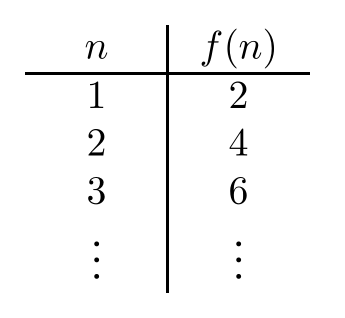
\includegraphics[width=6cm]{images/fn2n.png}
			
			{\bf Figura:} Visualização de $f$ através de uma tabela.
		\end{center}
	\end{frame}
	
	\begin{frame}{Método da diagonalização}
		\begin{block}{Considerações}
			\begin{itemize}
				\item Pode parecer contra-intuitivo, pois $P \subseteq \mathbb{N}$;  
				\item Mas é possível fazer a correspondência entre os conjuntos;  
				\item Logo, declaramos que esses conjuntos têm o mesmo tamanho.			
			\end{itemize}
		\end{block}  
		\begin{block}{Conjunto Contável}
			Um conjunto $A$ é {\bf contável} se é finito ou \\se tem o mesmo tamanho de $\mathbb{N}$.
		\end{block}
	\end{frame}
	
	\begin{frame}{Método da diagonalização}
		\begin{block}{Exemplo 2}
			Seja $\mathcal{Q} = \{ m / n$ | $m, n \in \mathbb{N} \}$ o conjunto dos racionais positivos.
		\end{block}  
		\begin{block}{$\mathcal{Q}$ é contável (curiosamente)} 
			Logo $\mathcal{Q}$ é finito ou tem o mesmo tamanho de $\mathbb{N}$.
		\end{block}
	\end{frame}
	
	\begin{frame}{Método da diagonalização}
		\begin{center}
			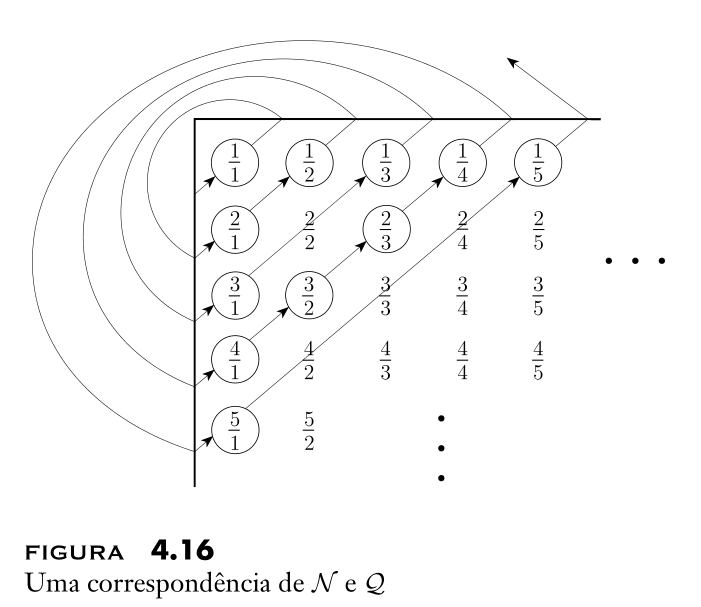
\includegraphics[width=8cm]{images/diagonal.png}
		\end{center}
	\end{frame}
	
	\begin{frame}{Método da diagonalização}
		\begin{block}{Considerações}
			\begin{itemize}
				\item Ao ver o exemplo de  $\mathcal{Q}$, há uma ligeira impressão de que qualquer conjunto é contável;  
				\item Mas existe conjuntos incontáveis;  
				\item Cantor provou que $\mathbb{R}$ é incontável introduzindo o \\método da diagonalização.
			\end{itemize}
		\end{block}  
		\begin{block}{Teorema 4.17}
			$\mathbb{R}$ é incontável.
		\end{block}
	\end{frame}

	\section{Conjunto Incontáveis}

	\begin{frame}{Conjuntos Incontáveis}
		\begin{block}{Teorema 4.17}
			$\mathbb{R}$ é incontável.
		\end{block} \pause
		\begin{block}{Ideia da Prova}
			\begin{itemize}
				\item De forma a mostrar que $\mathbb{R}$ é incontável, mostramos que nenhuma correspondência existe entre $\mathbb{N}$ e $\mathbb{R}$.
				\begin{itemize}
					\item Supomos, a princípio, que a correspondência $f$ existe.
					\item Logo após, apresentamos um valor $x \in \mathbb{R}$ que não está emparelhado com valor algum em $\mathbb{N}$ \\(o que indica um absurdo).				
				\end{itemize}
			\end{itemize}
		\end{block}
	\end{frame}
	
	\begin{frame}{Conjuntos Incontáveis}
		\begin{center}
			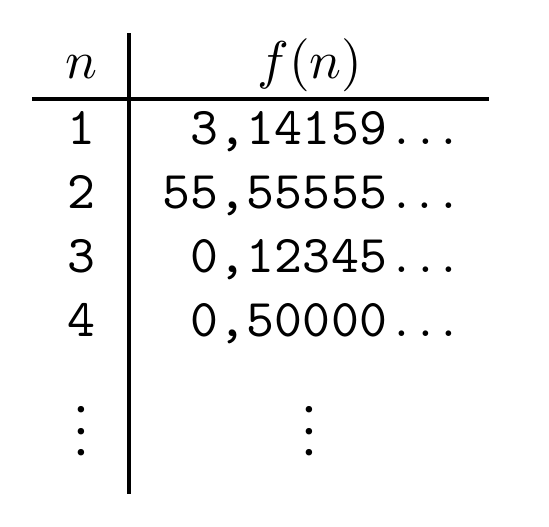
\includegraphics[width=6cm]{images/fHip.png}
			
			{\bf Figura:} Suposta correspondência $f$ entre $\mathbb{N}$ e $\mathbb{R}$.
		\end{center}
	\end{frame}
	
	\begin{frame}{Conjuntos Incontáveis}
		\begin{center}
			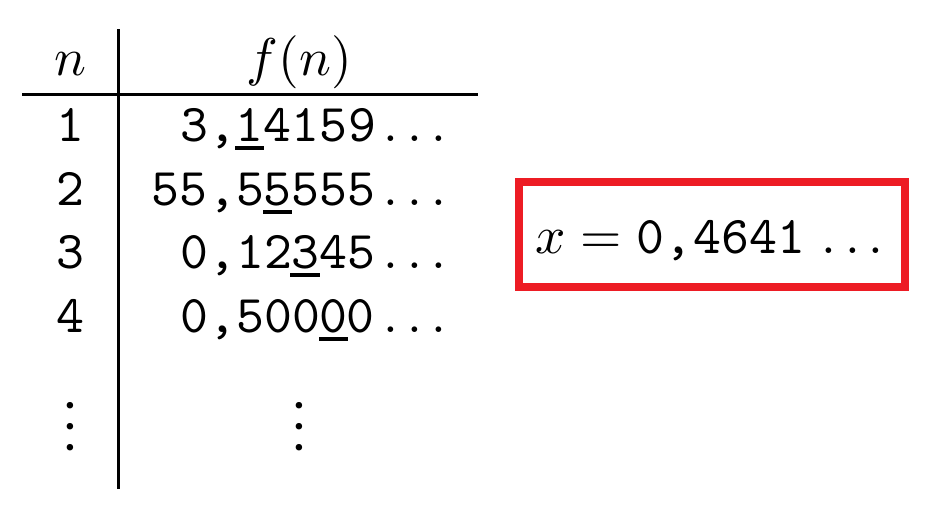
\includegraphics[width=9cm]{images/fHipX.png}
			
			{\bf Figura:} Construção de $x$ a partir da correspondência $f$.
		\end{center}
	\end{frame}
	
	\begin{frame}{Conjuntos Incontáveis}
		\begin{block}{Considerações}
			Apenas deve-se ter o cuidado de escolher dígitos para $x$ \\diferentes de 0 e 9, devido ao fato de 
			\begin{center}
				$3,999 \ldots = 4,000 \ldots$
			\end{center}
		\end{block}
	\end{frame}
	
	\begin{frame}{Conjuntos Incontáveis}
		\begin{exampleblock}{Corolário do Teorema 4.17}
			Algumas linguagens não são Turing-reconhecíveis.
		\end{exampleblock} \pause
		\begin{block}{Ideia da Prova}
			\begin{enumerate}
				\item Observar que o conjunto de todas as máquinas de Turing é contável; \pause
				\item Observar que o conjunto de todas as linguagens é incontável. \pause
				\item Como há mais linguagens do que máquinas de Turing, então algumas linguagens não podem ser Turing-reconhecíveis.
			\end{enumerate}
		\end{block}
	\end{frame}
	
	\begin{frame}{Conjuntos Incontáveis}
		\begin{block}{O conjunto de todas as máquinas de Turing é contável}
			\begin{itemize}
				\item $\Sigma^*$ é contável; \pause
				\item Cada máquina de Turing pode ser codificada em uma cadeia $\langle M \rangle$; \pause
				\item O conjunto $C$ de todas as máquinas de Turing pode ser representado por um conjunto de cadeias $\langle M \rangle$; \pause
				\item É possível enumerar $C$; \pause
				\item Logo $C$ é contável.
			\end{itemize}
		\end{block}
	\end{frame}

	\begin{frame}{Conjuntos Incontáveis}
		\begin{center}
			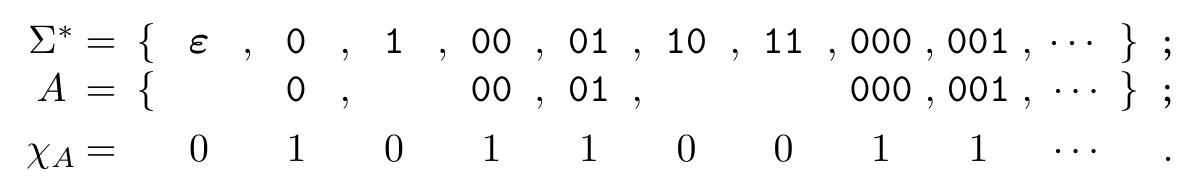
\includegraphics[width=11cm]{images/seqCar.png}
			
			{\bf Figura:} Construção de $\mathcal{X}A$ a partir da correspondência $\Sigma^*$.
		\end{center}
	\end{frame}
	
	\begin{frame}{Conjuntos Incontáveis}
		\begin{block}{O conjunto de todas as linguagens é incontável}
			\begin{itemize}
				\item O conjunto $B$ de todas as sequências binárias infinitas é incontável; \pause
				\item Qualquer linguagem pode ser descrita como uma sequência característica; \pause
				\item O conjunto $L$ de todas as linguagens podem ser representado por um conjunto de sequências \pause característica; \pause
				\item A função $f : L \rightarrow B$ \\(em que $f(A)$ é igual à sequência característica de $A$) \\é uma correspondência; \pause
				\item Logo, como $B$ é incontável, $L$ é incontável.
			\end{itemize}
		\end{block}
	\end{frame}
	
	\begin{frame}{Conjuntos Incontáveis}
		\begin{block}{Exercício}
			Mostrar que o problema da parada é indecidível.
		\end{block}
	\end{frame}
	
	\begin{frame}
		\titlepage
	\end{frame}
	
\end{document}